%# -*- coding: utf-8 -*-
% !TEX encoding = UTF-8 Unicode
\RequirePackage{fixltx2e}
\documentclass[aps,pre,12pt,preprint,onecolumn,showpacs,showkeys,UTF8]{revtex4-1}
\usepackage{ctex}
\usepackage{mathrsfs}
\usepackage{setspace,dcolumn}
\usepackage{subfigure}
\usepackage{graphicx,psfrag,epsfig}
\usepackage[font=small,format=plain,labelfont=bf,textfont=it,justification=raggedright,singlelinecheck=false]{caption}
\usepackage{amsmath,amsfonts,amssymb,amsthm,bm,upgreek}
\usepackage{geometry}
\usepackage[mathscr]{eucal}
\usepackage{titlesec}
\usepackage{tabularx}
\titleformat{\section}{\bf\fangsong\zihao{4}}{\thesection}{0.75em}{}
\geometry{top=2.54cm,bottom=2.54cm,left=3cm,right=3cm}
\renewcommand\appendixname{附录}
\renewcommand\abstractname{}%摘要
\renewcommand\tablename{表}
\renewcommand\figurename{图}
\makeatletter
\def\@keys@name{\songti\zihao{-4}{\bf 关键词:}}
\def\Received@name{\zihao{-5}{接收} }
\def\Revised@name{\zihao{-5}{修订} }
\def\Accepted@name{\zihao{-5}{采纳} }
\def\Published@name{\zihao{-4}{发表} }
\makeatother
\linespread{1.6}
\renewcommand{\labelenumi}{\alph{enumi}.}
\leftmargini=20mm

\begin{document}

\title{\bf\heiti\zihao{3}晶体的电光效应以及其应用\vspace{15mm}}
\author{\fangsong 乔颢\vspace{2mm}}
\affiliation{\songti\zihao{-4}北京大学物理学院2011级2班~~~~学号:1100011354 \vspace{2mm}}
\keywords{电光效应,磷酸二氚钾晶体,半波电压}
\email{1993422qsh@gmail.com; 18600200672}
\begin{abstract} 
	\vspace{10mm}
	\begin{spacing}{1.5}
		\songti\zihao{-4}本实验测量了电光晶体的半波电压为5368V,以及电光系数$r_{63}=17.19\times10^{-10} cm \cdot V^{-1}$。并且利用了这个电光晶体测量了云母样品两个轴的折射率差为0.0052。
	\end{spacing}
\end{abstract}

\maketitle

\section{引言}
当介质加上电场之后,其折射率发生变化的现象被称作电光效应。电场与折射率之间的关系可以用以下的公式所表示:

\begin{equation}
	n=n^0+nE_0+bE_0^2+\cdots
\end{equation}

其中由一次相$nE_0$引起的折射率变化被称为一次电光效应。本实验研究的就是KD*P(磷酸二氚钾)晶体的一次电光效应。本实验分别才用了三种不同的方法测量了晶体的半波电压值,得出了光点系数,并且用电光晶体做相位补偿器测量云母样品的相位差。

通过本实验,可以进一步的理解物理光学,晶体光学等相关知识,提高综合应用这些解决实际问题的能力。了解测量半波电压的多种方法,掌握测量晶体相位差的方法,学习光路中的调节技巧等等。

\section{实验原理}
KD*P为单轴晶体,其折射率椭球为:

\begin{equation}
	\frac{x^2+y^2}{n_o^2}+\frac{z^2}{n_e^2}=1
\end{equation}
当加上沿光轴方向的电场之后,KD*P晶体折射率椭球改变。重新选定长短轴之后依然可以写成折射率椭球的形式。可以得到旋转x,y坐标轴45$^\circ$之后,可以得到以下关系:
\begin{displaymath}
	\left\{\begin{array}{l}
		n_{x'}=n_o(1+n_o^2r_{63}E_x)^{-1/2} \\
		n_{y'}=n_o(1-n_o^2r_{63}E_x)^{-1/2} \\
		n_{z'}=n_e
	\end{array}\right.
\end{displaymath}
因为外场下折射率改变很小,可以展开。计算得到沿着x'和y'的光波会产生一个相位差。当产生相位差为$\pi$的话可以得到:
\begin{equation}
	r_{63}=\frac{\lambda}{2n_o^3V_\pi}
\end{equation}

\section{实验仪器和过程}
实验装置如图所示:
\begin{figure}[h]
	\begin{center}
		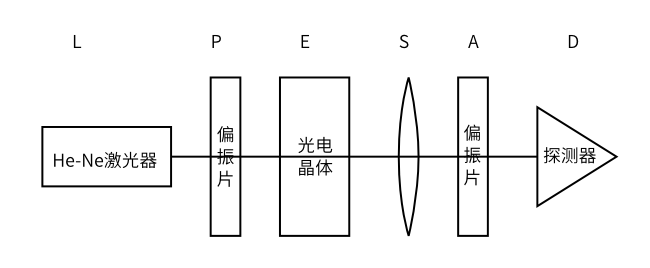
\includegraphics[width=0.7\textwidth]{pic1.png}
		\caption{\label{g:1}晶体电光效应研究装置图。He-Ne激光器出射波长为632.8nm,电光晶体E由四块晶体串联得到,总长度为6cm,样品为云母片,厚度为20$\mu m$。}
	\end{center}
\end{figure}
\subsection{调节光路}

由氦氖激光器发出的激光经过偏振片P形成偏振光,经过加入电压的电光晶体调整相位后进入样品,最后在经过偏振片测量偏振性,由探测器接受光。具体的实验步骤如下。

首先调节激光的水平。整激光的高度和仰角,使其入射到偏振片的一个固定位置,,移动偏振片和激光的距离,继续调整使得位置不变即可(远调仰角,近调高度)。随后任意制定偏振片P的指向,调整A使之偏振方向与P垂直,此时观察到消光现象。

随后使用锥光干涉的远离调节电光晶体的光轴与激光传播方向一致。细致调节电光晶体的位置,使得锥光干涉中的暗十字正交,并且似的亮度均匀。这样可以粗略的认为电光晶体的z轴摆放正确。随后调节偏振片P和A,使其与x,y平行。开始时P指向$0^\circ$,A指向$78^\circ$保持P方向不变,此时调整A的方向以及加在晶体上的电压U,使得电光探测器中得到的光功率最小。此后记录A偏转的角度为$44^\circ$,所以调整A和P方向,P顺时针旋转23度,A逆时针旋转23度即可。此时P和A就可以认为其与x,y平行,测量的电压为1255V。第一种测量方式得到半波电压为$U_\pi=5020V$。

\subsection{使用直流电压响应法测量半波电压}

随后在保持偏振方向(A,P垂直)的情况使用直流电压响应法测量半波电压。此时有输入输出光强的关系满足:
\begin{equation}
	I_{output}=\frac{I_{input}}{2}(1-\cos \Phi)
\end{equation}
所以可以通过测量输出功率和电压的关系得到半波电压。测量结果如下:
\begin{table}[ht]
	\centering
	\begin{tabular}{m{3cm}<{\centering}m{3cm}<{\centering}m{3cm}<{\centering}m{3cm}<{\centering}}
		\hline
		\hline
		U/V	&	P/mW	&	U/V	&	P/mW	\\
		\hline
-1450	&	1.242	&	600	&	0.679	\\
-1400	&	1.246	&	700	&	0.863	\\
-1350	&	1.239	&	800	&	1.03	\\
-1300	&	1.22	&	900	&	1.202	\\
-1200	&	1.194	&	1000	&	1.364	\\
-1000	&	0.96	&	1100	&	1.447	\\
-800	&	0.667	&	1150	&	1.487	\\
-600	&	0.351	&	1200	&	1.517	\\
-400	&	0.131	&	1225	&	1.525	\\
-200	&	0.029	&	1250	&	1.53	\\
-100	&	0.015	&	1275	&	1.539	\\
0	&	0.029	&	1300	&	1.536	\\
100	&	0.071	&	1325	&	1.537	\\
200	&	0.132	&	1350	&	1.536	\\
300	&	0.227	&	1375	&	1.525	\\
400	&	0.35	&	1400	&	1.512	\\
500	&	0.516	&	-	&	-	\\
\hline
	\end{tabular}
	\caption{电光晶体调相后,经过偏振片输出光功率和电光晶体所加电压和关系表。其中的电压是加载1/4晶体上的电压。}
	\label{tab:table1}
\end{table}
\begin{figure}[ht]
	\begin{center}
		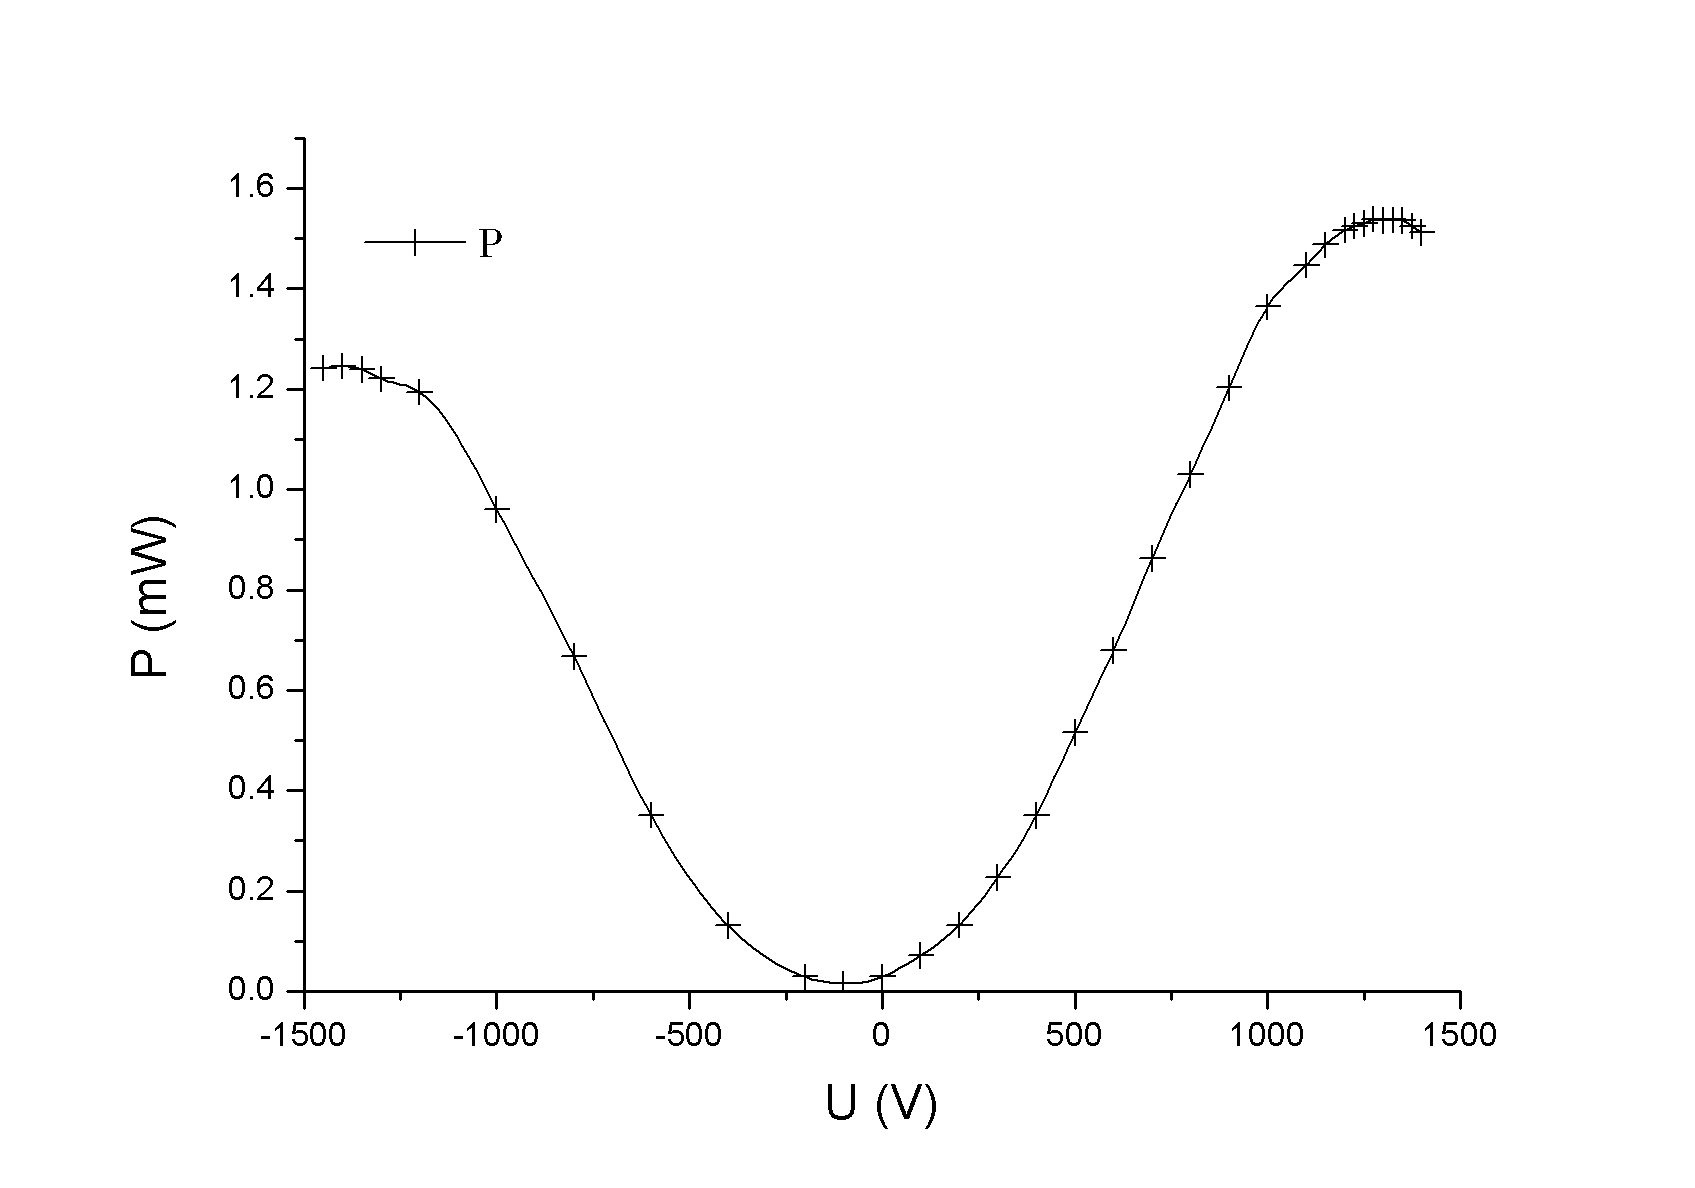
\includegraphics[width=0.7\textwidth]{pic2.png}
	\end{center}
	\caption{电光晶体所加电压与光路输出光功率关系图。其中的电压是加载1/4晶体上的电压。}
	\label{fig:fig2}
\end{figure}
根据数据可以得到对应的半波电压$U_\pi=5500V$。这里和上一种方法测量得到的结果相差很大,原因在于上一种测量方式并没有考虑其零点,也就是说在没有添加电压的时候,本身晶体就会产生一定的相位差,这一点上一个测量中没有考虑到。

\subsection{使用调制法测量半波电压}

保持A与P的垂直,在晶体的直流电压上增加一个合适的基频信号。当直流偏置电压满足一定条件后,输出的光信号是一个倍频信号。此时的直流偏置电压所产生相位差$\Phi=0$或者$\Phi=\pi$。所以根据这一点可以测量得到半波电压。记录当输入的频率为1.118kHz的时候,P垂直于A,此时电压为-82V的时候出现了倍频现象。调整使得A平行于P,测量可以得到当电压为1260V时出现了倍频。所以可以的得到$U_\pi=(1260+115)\times4=5368V$。即半波电压为5368V。

带入计算可以得到
\begin{equation}
	r_{64}=\frac{\lambda}{2n_o^3U_\pi}=17.19\times10^{-10} cm \cdot V^{-1}
\end{equation}
这里的$n_o$是查表得到的1.5079。计算得到的$r_{63}$与理论得到的值十分的接近。此时可以验证,当加上U=5368V的电压后,折射率椭球的偏移$\Delta n$的确很小,为:
\begin{equation}
	\Delta n=\frac{1}{2}n_o^3r_{63}E_z=3.0\times10^{-6}
\end{equation}
的确是可以直接展开为一阶项而忽略二阶项。

\subsection{测量样品的相位差和折射率差。}

接下来是利用电光晶体来测量云母片样品的相位差以及折射率差。首先选定A与P垂直,调整直流偏置使得出射光功率最小,出现二倍频,此时V=-140V。放入样品,调整样品的指向,使得倍频出现,此时有云母片的一个光轴与A的偏振方向一致。随后旋转样品45度,调整电压至二倍频再次出现。此时电压为324V。所以可以得到电压差为464V即相位移动了$\Phi=0.346\pi$。即此云母片的相位差为$0.346\Pi$。带入公式可以得到折射率差为:

\begin{equation}
	\Delta n = \frac{\Phi \lambda}{2 D} = 0.0055
\end{equation}

使用A平行于P测量可以得到电压差为927V,可以得到相位移动了$\Phi=0.31\pi$,所以得到了折射率差为0.0049,两个测量方式差别不大,取平均值可以得到较正确的解。误差来源可能来自于样品光轴方向并不是严格的与A偏振方向一致。

\section{结论}

KD*P电光晶体的半波电压用不同的测量方式分别测量得到 5020V, 5500V, 5368V。其中5368V是比较精确的值。由此测量得到的电光系数为$r_{63}=17.19\times10^{-10} cm \cdot V^{-1}$。

测量的样品相位差为$0.328\pi$,折射率差0.0052。


\section{致谢} 
感谢蒋莹莹老师的指导,以及贾春燕,冉书能老师的技术支持。

\begin{thebibliography}{}
	\bibitem{Book} 吴思成,王祖铨~2010 近代物理实验(第三版)(北京:高等教育出版社)第165页.%
%
\end{thebibliography}

\clearpage
\appendix
\section{思考题} 

1、 他们不同在于如何精确的确定光强极大和光强极小。前两种测量方式是直接测量光强来确定电压差,而第三种方法则是使用了一种间接的方法来较精确的确定极大极小点。所以第三种更为精确。

2、光学调制器可以由本实验中的晶体组成,他可以调整相位差。

3、电光晶体与激光不平行可以利用锥光干涉进行检验。不平行的话会使得折射率椭球并不正对激光光路,从而使得调相引入误差,测量得到的结果也会不准确。与PA不平行一样的会使得调相的两个分量本身就有相位差从而影响结果。

4、这样做更为精确,而其他的测量手段可能精度不够好。
\end{document} 
